\documentclass[
  shownotes,
  xcolor={svgnames},
  hyperref={colorlinks,citecolor=DarkBlue,linkcolor=DarkRed,urlcolor=DarkBlue}
  , aspectratio=169]{beamer}
\usepackage{animate}
\usepackage{amsmath}
\usepackage{amsfonts}
\usepackage{amssymb}
\usepackage{pifont}
\usepackage{mathpazo}
%\usepackage{xcolor}
\usepackage{multimedia}
\usepackage{fancybox}
\usepackage[para]{threeparttable}
\usepackage{multirow}
\setcounter{MaxMatrixCols}{30}
\usepackage{subcaption}
\usepackage{graphicx}
\usepackage{lscape}
\usepackage[compatibility=false,font=small]{caption}
\usepackage{booktabs}
\usepackage{ragged2e}
\usepackage{chronosys}
\usepackage{appendixnumberbeamer}
\usepackage{animate}
\setbeamertemplate{caption}[numbered]
\usepackage{color}
%\usepackage{times}
\usepackage{tikz}
\usepackage{comment} %to comment
%% BibTeX settings
\usepackage{natbib}
\bibliographystyle{apalike}
\bibpunct{(}{)}{,}{a}{,}{,}
\setbeamertemplate{bibliography item}{[\theenumiv]}

% Defines columns for bespoke tables
\usepackage{array}
\newcolumntype{L}[1]{>{\raggedright\let\newline\\\arraybackslash\hspace{0pt}}m{#1}}
\newcolumntype{C}[1]{>{\centering\let\newline\\\arraybackslash\hspace{0pt}}m{#1}}
\newcolumntype{R}[1]{>{\raggedleft\let\newline\\\arraybackslash\hspace{0pt}}m{#1}}


\usepackage{xfrac}


\usepackage{multicol}
\setlength{\columnsep}{0.5cm}

% Theme and colors
\usetheme{Boadilla}

% I use steel blue and a custom color palette. This defines it.
\definecolor{andesred}{HTML}{af2433}

% Other options
\providecommand{\U}[1]{\protect\rule{.1in}{.1in}}
\usefonttheme{serif}
\setbeamertemplate{itemize items}[default]
\setbeamertemplate{enumerate items}[square]
\setbeamertemplate{section in toc}[circle]

\makeatletter

\definecolor{mybackground}{HTML}{82CAFA}
\definecolor{myforeground}{HTML}{0000A0}

\setbeamercolor{normal text}{fg=black,bg=white}
\setbeamercolor{alerted text}{fg=red}
\setbeamercolor{example text}{fg=black}

\setbeamercolor{background canvas}{fg=myforeground, bg=white}
\setbeamercolor{background}{fg=myforeground, bg=mybackground}

\setbeamercolor{palette primary}{fg=black, bg=gray!30!white}
\setbeamercolor{palette secondary}{fg=black, bg=gray!20!white}
\setbeamercolor{palette tertiary}{fg=white, bg=andesred}

\setbeamercolor{frametitle}{fg=andesred}
\setbeamercolor{title}{fg=andesred}
\setbeamercolor{block title}{fg=andesred}
\setbeamercolor{itemize item}{fg=andesred}
\setbeamercolor{itemize subitem}{fg=andesred}
\setbeamercolor{itemize subsubitem}{fg=andesred}
\setbeamercolor{enumerate item}{fg=andesred}
\setbeamercolor{item projected}{bg=gray!30!white,fg=andesred}
\setbeamercolor{enumerate subitem}{fg=andesred}
\setbeamercolor{section number projected}{bg=gray!30!white,fg=andesred}
\setbeamercolor{section in toc}{fg=andesred}
\setbeamercolor{caption name}{fg=andesred}
\setbeamercolor{button}{bg=gray!30!white,fg=andesred}



\usepackage{fancyvrb}
\newcommand{\VerbBar}{|}
\newcommand{\VERB}{\Verb[commandchars=\\\{\}]}
\DefineVerbatimEnvironment{Highlighting}{Verbatim}{commandchars=\\\{\}}
% Add ',fontsize=\small' for more characters per line
\usepackage{framed}
\definecolor{shadecolor}{RGB}{248,248,248}
\newenvironment{Shaded}{\begin{snugshade}}{\end{snugshade}}
\newcommand{\AlertTok}[1]{\textcolor[rgb]{0.94,0.16,0.16}{#1}}
\newcommand{\AnnotationTok}[1]{\textcolor[rgb]{0.56,0.35,0.01}{\textbf{\textit{#1}}}}
\newcommand{\AttributeTok}[1]{\textcolor[rgb]{0.77,0.63,0.00}{#1}}
\newcommand{\BaseNTok}[1]{\textcolor[rgb]{0.00,0.00,0.81}{#1}}
\newcommand{\BuiltInTok}[1]{#1}
\newcommand{\CharTok}[1]{\textcolor[rgb]{0.31,0.60,0.02}{#1}}
\newcommand{\CommentTok}[1]{\textcolor[rgb]{0.56,0.35,0.01}{\textit{#1}}}
\newcommand{\CommentVarTok}[1]{\textcolor[rgb]{0.56,0.35,0.01}{\textbf{\textit{#1}}}}
\newcommand{\ConstantTok}[1]{\textcolor[rgb]{0.00,0.00,0.00}{#1}}
\newcommand{\ControlFlowTok}[1]{\textcolor[rgb]{0.13,0.29,0.53}{\textbf{#1}}}
\newcommand{\DataTypeTok}[1]{\textcolor[rgb]{0.13,0.29,0.53}{#1}}
\newcommand{\DecValTok}[1]{\textcolor[rgb]{0.00,0.00,0.81}{#1}}
\newcommand{\DocumentationTok}[1]{\textcolor[rgb]{0.56,0.35,0.01}{\textbf{\textit{#1}}}}
\newcommand{\ErrorTok}[1]{\textcolor[rgb]{0.64,0.00,0.00}{\textbf{#1}}}
\newcommand{\ExtensionTok}[1]{#1}
\newcommand{\FloatTok}[1]{\textcolor[rgb]{0.00,0.00,0.81}{#1}}
\newcommand{\FunctionTok}[1]{\textcolor[rgb]{0.00,0.00,0.00}{#1}}
\newcommand{\ImportTok}[1]{#1}
\newcommand{\InformationTok}[1]{\textcolor[rgb]{0.56,0.35,0.01}{\textbf{\textit{#1}}}}
\newcommand{\KeywordTok}[1]{\textcolor[rgb]{0.13,0.29,0.53}{\textbf{#1}}}
\newcommand{\NormalTok}[1]{#1}
\newcommand{\OperatorTok}[1]{\textcolor[rgb]{0.81,0.36,0.00}{\textbf{#1}}}
\newcommand{\OtherTok}[1]{\textcolor[rgb]{0.56,0.35,0.01}{#1}}
\newcommand{\PreprocessorTok}[1]{\textcolor[rgb]{0.56,0.35,0.01}{\textit{#1}}}
\newcommand{\RegionMarkerTok}[1]{#1}
\newcommand{\SpecialCharTok}[1]{\textcolor[rgb]{0.00,0.00,0.00}{#1}}
\newcommand{\SpecialStringTok}[1]{\textcolor[rgb]{0.31,0.60,0.02}{#1}}
\newcommand{\StringTok}[1]{\textcolor[rgb]{0.31,0.60,0.02}{#1}}
\newcommand{\VariableTok}[1]{\textcolor[rgb]{0.00,0.00,0.00}{#1}}
\newcommand{\VerbatimStringTok}[1]{\textcolor[rgb]{0.31,0.60,0.02}{#1}}
\newcommand{\WarningTok}[1]{\textcolor[rgb]{0.56,0.35,0.01}{\textbf{\textit{#1}}}}
\usepackage{graphicx}
\makeatletter

\makeatother


%%%%%%%%%%%%%%% BEGINS DOCUMENT %%%%%%%%%%%%%%%%%%

\begin{document}

\title{Lecture 2:  Sobreajuste \&  Validación Cruzada}
\subtitle{Aprendizaje y Minería de Datos para los Negocios}
\date{\today}

\author[Sarmiento-Barbieri]{Ignacio Sarmiento-Barbieri}
\institute[Uniandes]{Universidad de los Andes}


\begin{frame}[noframenumbering]
\maketitle
\end{frame}

%%%%%%%%%%%%%%%%%%%%%%%%%%%%%%%%%%%
%       Motivation              %
% What is the question?
% Why do we care?
% What is new?
% What do you find?
%%%%%%%%%%%%%%%%%%%%%%%%%%%%%%%%%%%




\begin{frame}
\frametitle{Agenda}

\tableofcontents


\end{frame}
%----------------------------------------------------------------------%
\section{Recap} 
%----------------------------------------------------------------------%
%----------------------------------------------------------------------%
\subsection{La máquina de aprender y Modelos Lineales} 
%----------------------------------------------------------------------%
\begin{frame}
\frametitle{¿Qué es la máquina de aprender?}

\begin{itemize}
  \item El aprendizaje de máquinas es una rama de la informática y la estadística, encargada de desarrollar algoritmos para predecir los resultados $y$ a partir de las variables observables $X$.
  \medskip
  \item La parte de aprendizaje proviene del hecho de que no especificamos cómo exactamente la computadora debe predecir $y$ a partir de $X$.
  \medskip
   \item Esto queda como un problema empírico que la computadora puede "aprender".
   \medskip
  \item En general, esto significa que nos abstraemos del modelo subyacente, el enfoque es muy pragmático
  
  \bigskip
  \bigskip

  \pause
  \begin{quote}
  \centering
  \bf ``Lo que sea que funciona, funciona...''
  \end{quote}
\end{itemize}

\end{frame}
%----------------------------------------------------------------------%
\begin{frame}
\frametitle{Predicción y Error Predictivo}


\begin{itemize}
  \item El objetivo es predecir $y$ dadas otras variables $X$. Ej: precio vivienda dadas las características
  \bigskip
  \item Asumimos que el link entre $y$ and $X$ esta dado por el modelo:
\end{itemize}
\bigskip
\begin{align}
  y = f(X) + u
\end{align}
\bigskip
\begin{itemize}
  \item donde $f(X)$ es cualquier función, 
  \bigskip
  \item  $u$ una variable aleatoria no observable $E(u)=0$ and $V(u) = \sigma^2$
\end{itemize}


\end{frame}

%----------------------------------------------------------------------%
\begin{frame}
\frametitle{Predicción y Error Predictivo}

\begin{itemize}
  \item En la práctica no conocemos $f(X)$
  \medskip
  \item Es necesario estimarla $\hat y = \hat f(X)$ 
  \medskip
  \item La medida de cuan bien funciona nuestro modelo es $MSE(y)= \frac{1}{n} \sum_{i=1}^n (y_i - \hat{y} )^2$
  \medskip
  \item Notemos que podemos descomponer el $MSE$ en dos partes
\end{itemize}

\begin{align}
  MSE (  y )  &= MSE(\hat f) + \sigma^2  
\end{align}
\medskip
\begin{itemize}
  \item  el error de estimar $f$ con $\hat f$. (\emph{reducible})
  \item  el error de no observar $u$. (\emph{irreducible})
\end{itemize}

\medskip

\end{frame}

%----------------------------------------------------------------------%
\begin{frame}
\frametitle{Predicción y Error Predictivo}

\begin{itemize}
  \item Descomponiendo un poco más:
  


\medskip

\begin{align}
  Err (  Y )  &= MSE(\hat f) + \sigma^2  \\
                 &= Bias^2(\hat f) + V(\hat f) +  Irreducible\,Error
\end{align}
\medskip

\item Este resultado es muy importante,  
\begin{itemize}
\item Aparece el  dilema entre sesgo y varianza
\end{itemize}
\end{itemize}
\end{frame}


%----------------------------------------------------------------------%
\begin{frame}
\frametitle{Prediction Error}

\begin{figure}[H] \centering
  \centering
  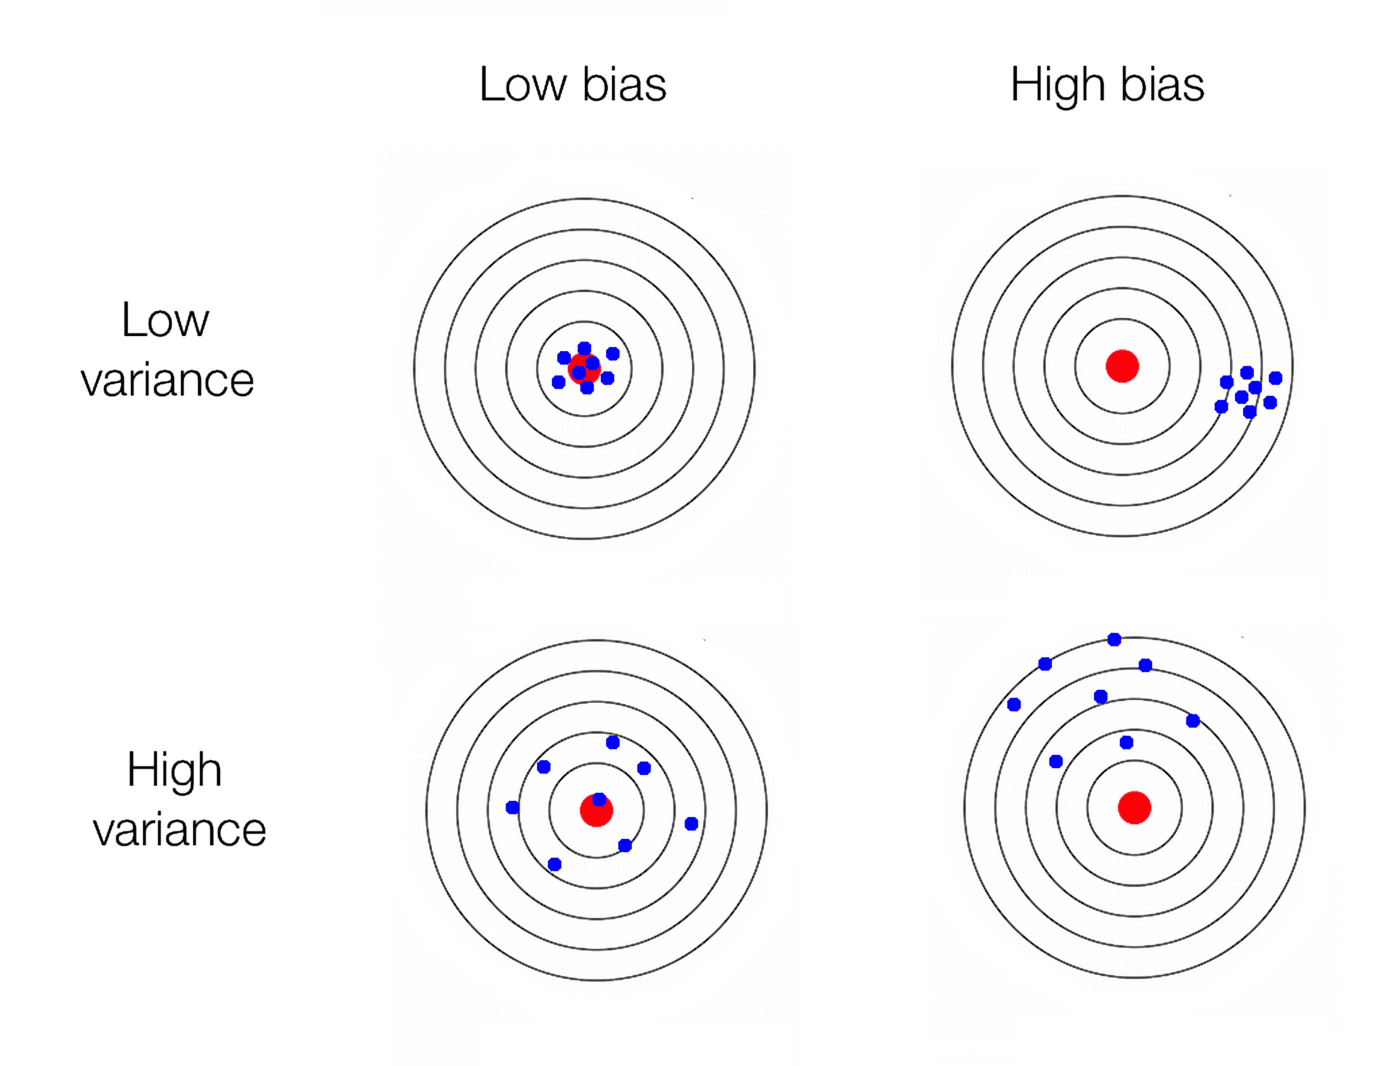
\includegraphics[scale=0.15]{figures/medium_bias_variance}
  \\
  \tiny
  Source: https://tinyurl.com/y4lvjxpc
\end{figure}


\end{frame}

%----------------------------------------------------------------------%
\begin{frame}[fragile]
\frametitle{Dilema sesgo/varianza}

\begin{itemize}
  \item El secreto de ML: admitiendo un poco de sesgo podemos tener ganancias importantes en varianza

\end{itemize}

\pause
\begin{figure}[H] \centering
  \centering
  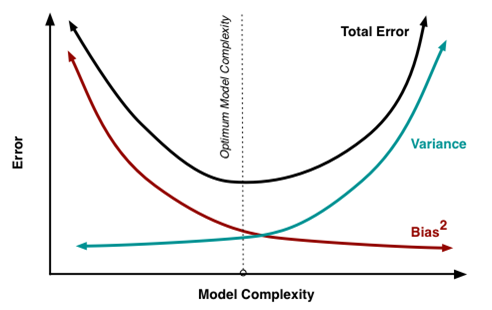
\includegraphics[scale=0.50]{figures/medium_bias_variance_trade_off.png}
  \\
  \tiny
  Source: https://tinyurl.com/y4lvjxpc
\end{figure}



\end{frame}

%----------------------------------------------------------------------%
\begin{frame}
\frametitle{Predicción y regresión lineal}

\begin{itemize}


\item El problema es:
\medskip
\begin{align}
y=f(X)+u
\end{align}

\item proponemos que:
\begin{align}
  f(X) = \beta_0 + \beta_1 X_1 + \dots + \beta_p X_p 
\end{align}

\item El problema se reduce a encontrar los $\beta$s
  \begin{itemize}
    \footnotesize
    \item Un camino es OLS
  \end{itemize}  
\end{itemize}
\end{frame}
%----------------------------------------------------------------------%
\begin{frame}
\frametitle{Predicción y regresión lineal}

\begin{itemize}
  \item Y el dilema sesgo varianza?
  \pause
  \item Bajo los supuestos clásicos (Gauss-Markov) el estimador de OLS es insesgado:

\medskip
\begin{align}
  E( X \hat \beta)&= E(\hat{\beta}_1 + \hat{\beta}_2 X_2 + \dots + \hat{\beta}_p X_p) \\ 
  &= E(\hat{\beta}_1) + E(\hat{\beta}_2) X_2 + \dots + E(\hat{\beta}_p) X_p  \\ 
  &= X \beta
\end{align}
\medskip

\item  $MSE(\hat y)$ se reduce a  $V(\hat \beta)$

\end{itemize}

\end{frame}

%----------------------------------------------------------------------%
\begin{frame}
\frametitle{Complejidad y compensación de varianza/sesgo}

\begin{itemize}
\item En la econometría clásica, la elección de modelos se resume a elegir entre modelos más pequeños y más grandes.
\item Considere los siguientes modelos para estimar  $y$:

\end{itemize}



\begin{minipage}[t]{0.48\linewidth}

          \begin{equation} 
          y=\beta_1 X_1 + u_1 \nonumber
          \end{equation}
        \begin{itemize}
          \item $\hat \beta^{(1)}_1$ el estimador de OLS $y$ on $X_1$
          \medskip
          \item La predicción es:
        \end{itemize}
        \bigskip
          \begin{equation}\label{eq:3_2_3}
          \hat{y}^{(1)}=\hat{\beta}^{(1)}_1 X_1 \nonumber
          \end{equation}
    
    \end{minipage}
    \hfill
    \begin{minipage}[t]{0.48\linewidth}%
        

        \begin{equation}
          y=\beta_1 X_1 + \beta_2 X_2 + u_2 \nonumber
        \end{equation}
      \begin{itemize}
          \item  $\hat \beta^{(2)}_1$ y $\hat \beta^{(2)}_2$ con $\beta_1$ y $\beta_2$ los el estimador de OLS de $y$ en $X_1$ y $X_2$. 
          \item La predicción es:
      \end{itemize}

      \begin{equation}\label{eq:3_2_4}
      \hat{y}^{(2)}=\hat{\beta}^{(2)}_1 X_1 + \hat{\beta}^{(2)}_2 X_2  \nonumber
      \end{equation}

    \end{minipage}
 
\end{frame}


%----------------------------------------------------------------------%
\begin{frame}
\frametitle{Complejidad y compensación de varianza/sesgo}

\begin{itemize}
  \item Una discusión importante en la econometría clásica es la de la omisión de variables relevantes frente a la inclusión de variables irrelevantes. 
  \medskip
  \begin{itemize}
    \item Si el modelo (1) es verdadero entonces estimar el modelo más grande (2) conduce a estimadores ineficientes aunque no sesgados debido a que incluyen innecesariamente $X_2$. 
    \medskip
    \item Si el modelo (2) se verdadero, estimar el modelo más pequeño (1) conduce a una estimación de menor varianza pero sesgada si $ X_1 $ también se correlaciona con el regresor omitido $X_2$. 
  \end{itemize}
  \medskip
  \item Esta discusión de pequeño vs grande siempre es con respecto a un modelo que se supone es verdadero.
  \medskip
\item  Pero en la práctica el modelo verdadero es desconocido!!!

\end{itemize}


\end{frame}

%----------------------------------------------------------------------%
\begin{frame}
\frametitle{Complejidad y compensación de varianza/sesgo}


\begin{itemize}
  \item Elegir entre modelos implica un dilema {\it sesgo/varianza}
  \medskip
\item La econometría clásica tiende a resolver este dilema abruptamente, 
  \begin{itemize}
    \item  requiriendo una estimación no sesgada y, por lo tanto, favoreciendo modelos más grandes para evitar sesgos
  \end{itemize}
\medskip
\item En esta configuración simple, los modelos más grandes son "más complejos", por lo que los modelos más complejos están menos sesgados pero son más ineficientes. 
\medskip
\item Por lo tanto, en este marco muy simple, la complejidad se mide por el número de variables explicativas.
\medskip
\item Una idea central en el aprendizaje automático es generalizar la idea de complejidad, 
  \begin{itemize}
    \item Nivel óptimo de complejidad, es decir, modelos cuyo sesgo y varianza conducen al menor MSE.
  \end{itemize}
\end{itemize}

\end{frame}

%----------------------------------------------------------------------%
\section{Overfit}
%----------------------------------------------------------------------%
\begin{frame}[fragile]
\frametitle{Overfit}


        \begin{figure}[H] \centering
            \captionsetup{justification=centering}
              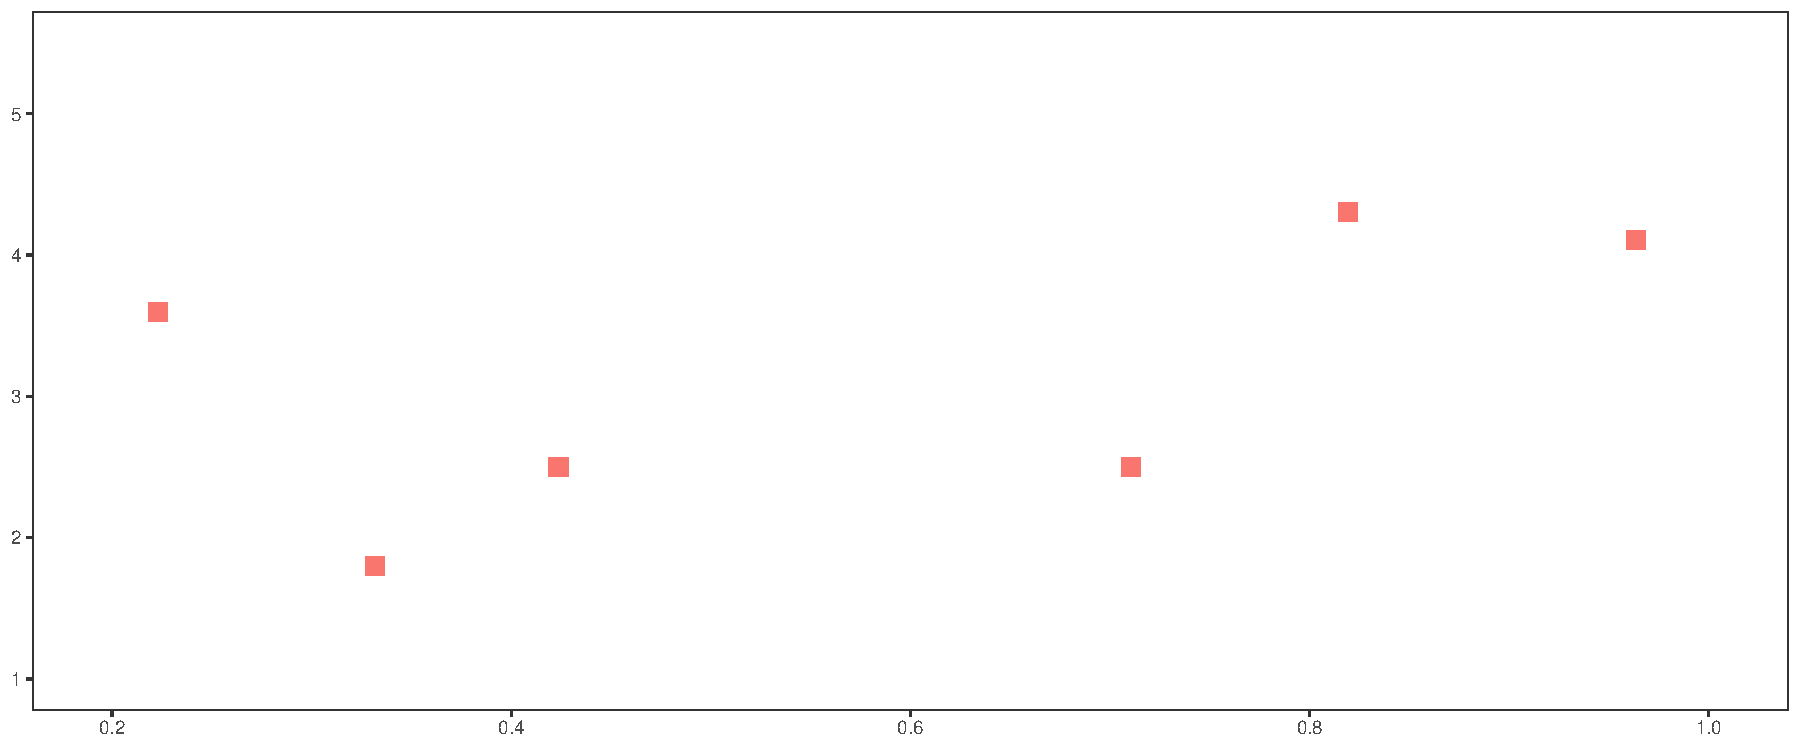
\includegraphics[scale=0.4]{figures/fig_1a.pdf}
 \end{figure}

\end{frame}

%----------------------------------------------------------------------%
\begin{frame}[fragile, noframenumbering]
\frametitle{Overfit}


        \begin{figure}[H] \centering
            \captionsetup{justification=centering}
              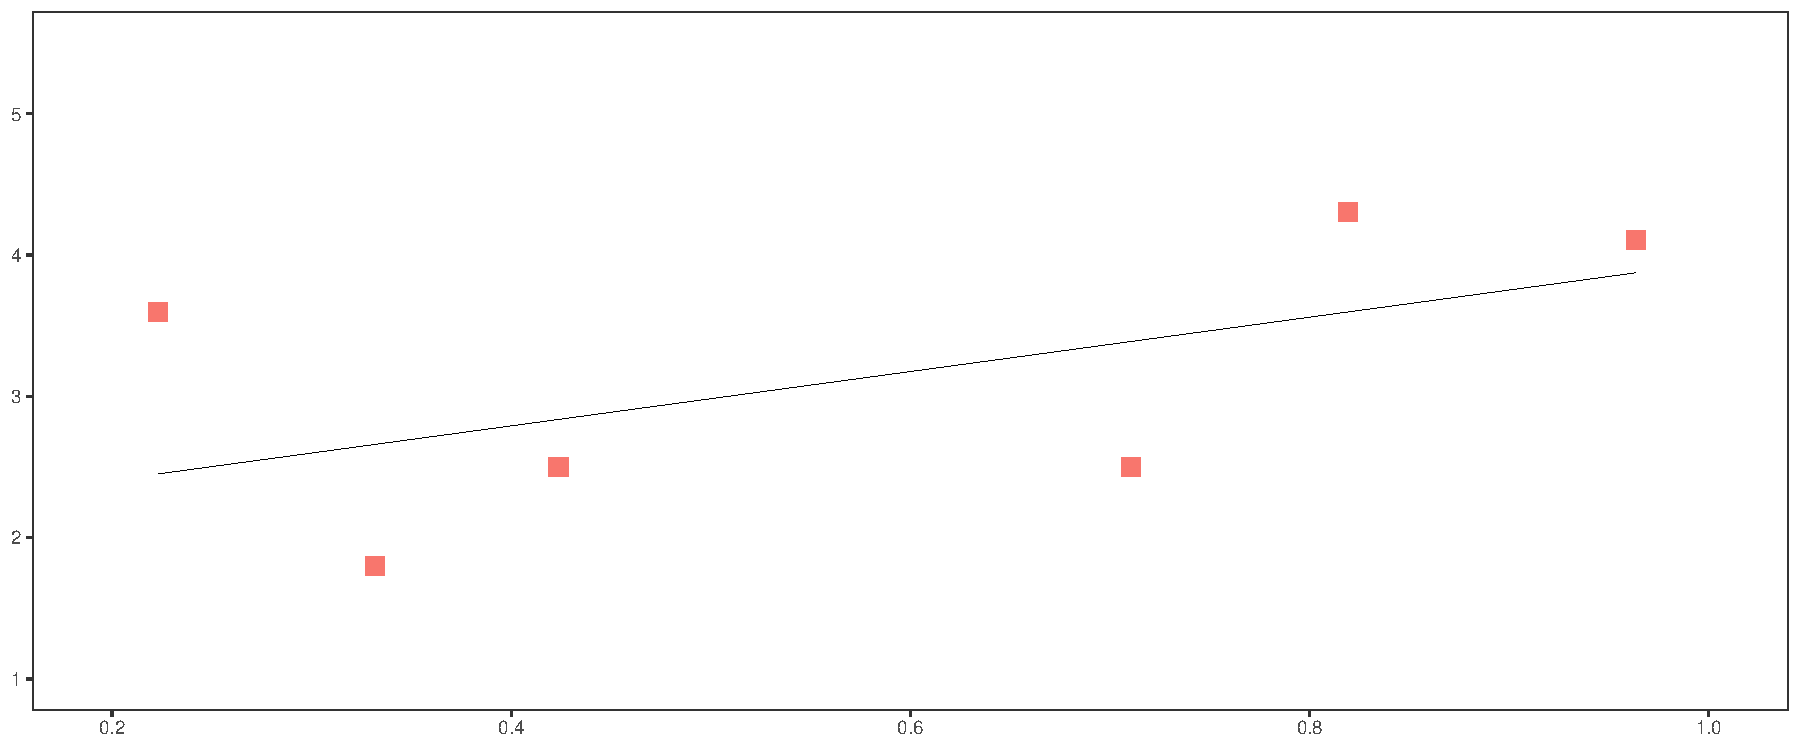
\includegraphics[scale=0.4]{figures/fig_1b.pdf}
 \end{figure}

\end{frame}
%----------------------------------------------------------------------%
\begin{frame}[fragile, noframenumbering]
\frametitle{Overfit}


        \begin{figure}[H] \centering
            \captionsetup{justification=centering}
              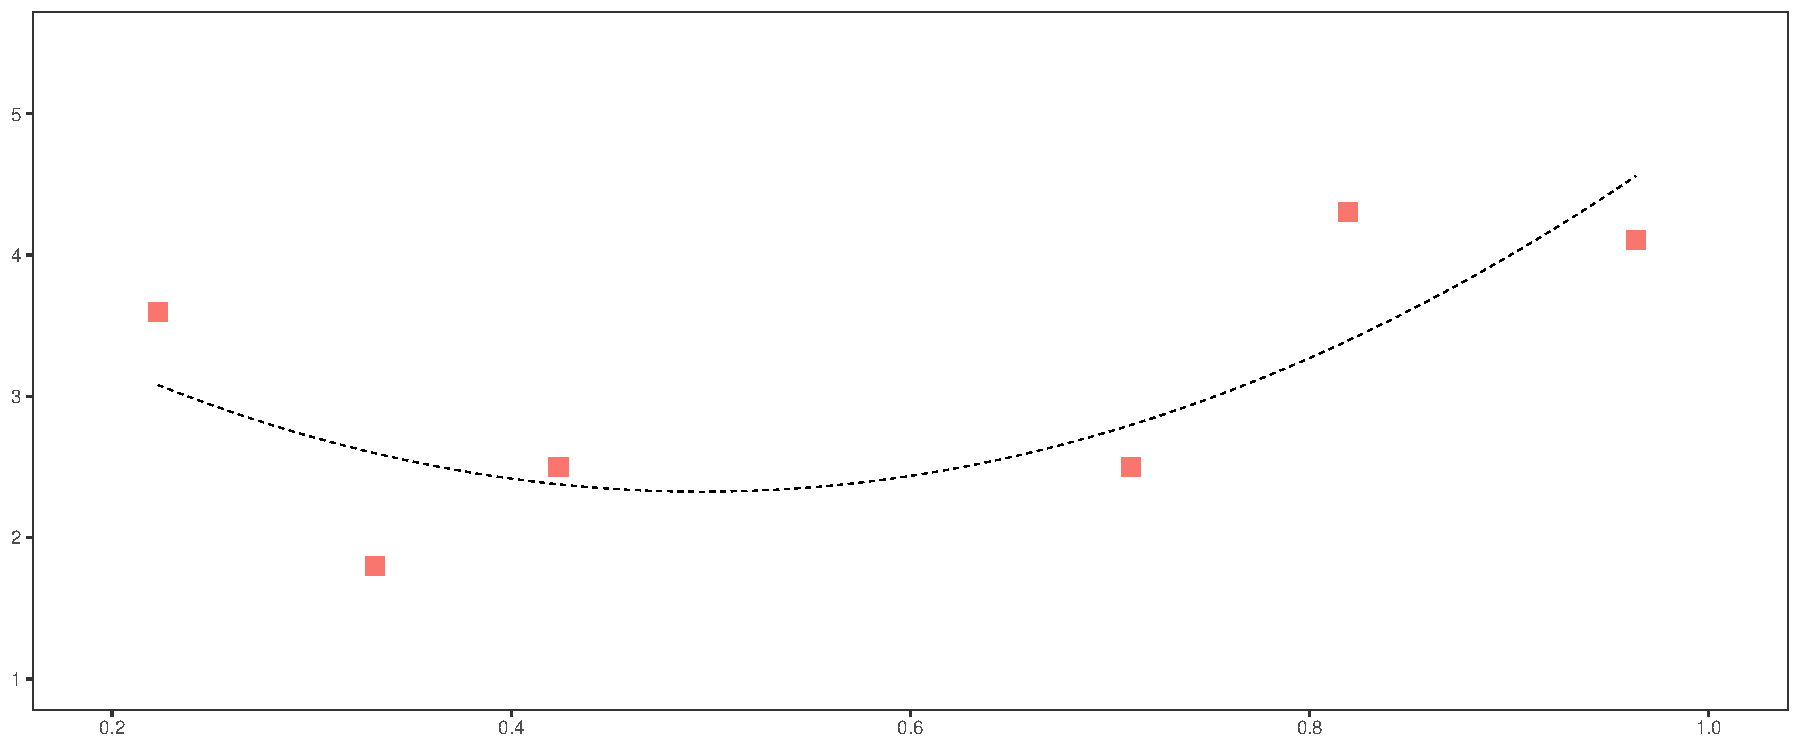
\includegraphics[scale=0.4]{figures/fig_1c.pdf}
 \end{figure}

\end{frame}

%----------------------------------------------------------------------%
\begin{frame}[fragile, noframenumbering]
\frametitle{Overfit}


        \begin{figure}[H] \centering
            \captionsetup{justification=centering}
              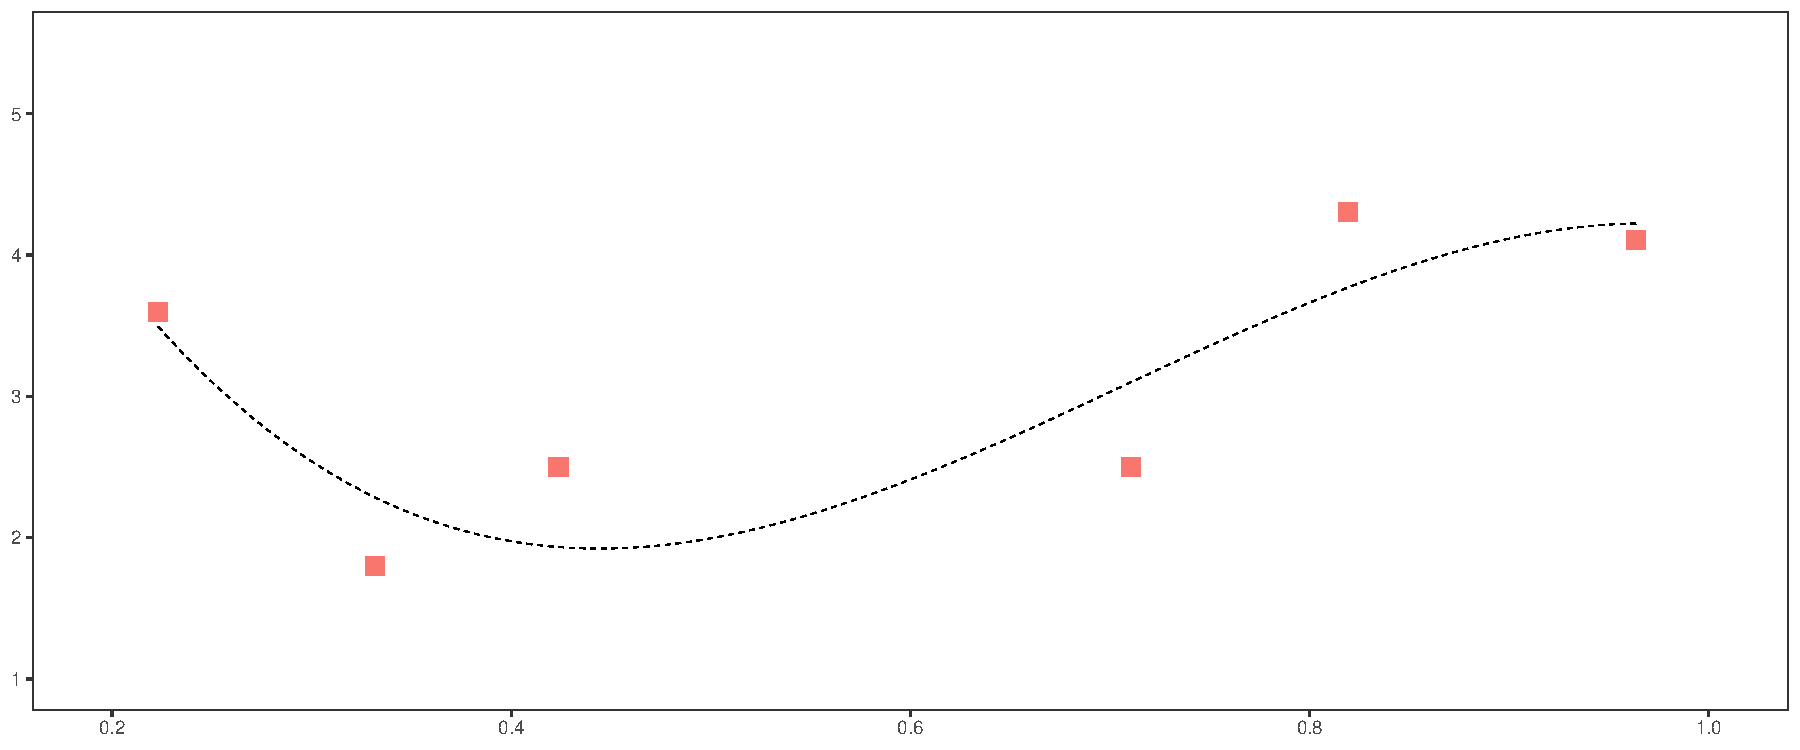
\includegraphics[scale=0.4]{figures/fig_1d.pdf}
 \end{figure}

\end{frame}
%----------------------------------------------------------------------%
\begin{frame}[fragile, noframenumbering]
\frametitle{Overfit}


        \begin{figure}[H] \centering
            \captionsetup{justification=centering}
              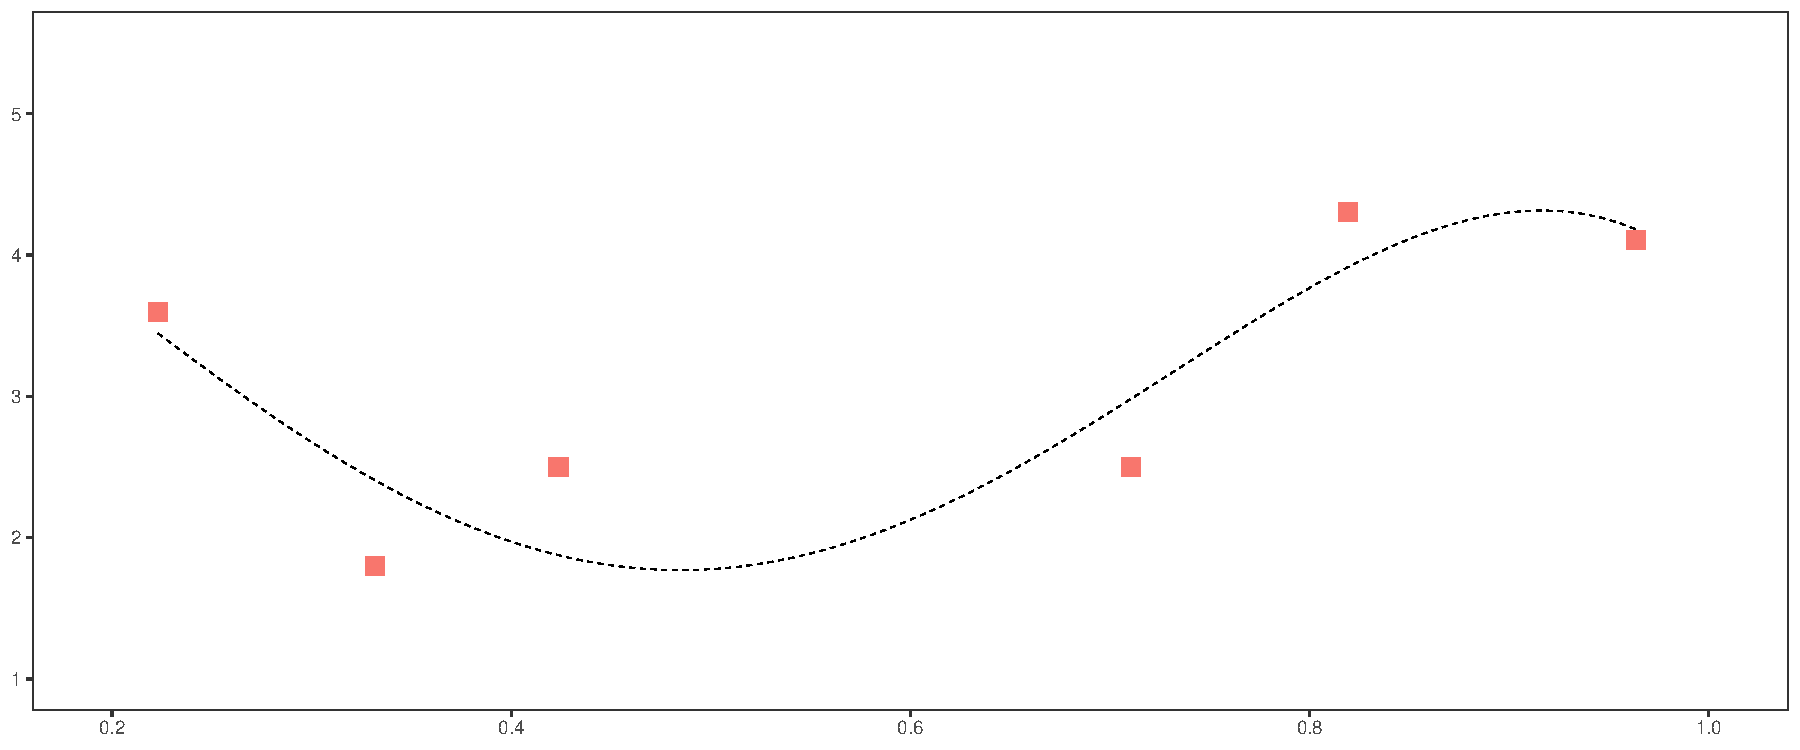
\includegraphics[scale=0.4]{figures/fig_1e.pdf}
 \end{figure}

\end{frame}
%----------------------------------------------------------------------%
\begin{frame}[fragile, noframenumbering]
\frametitle{Overfit}


        \begin{figure}[H] \centering
            \captionsetup{justification=centering}
              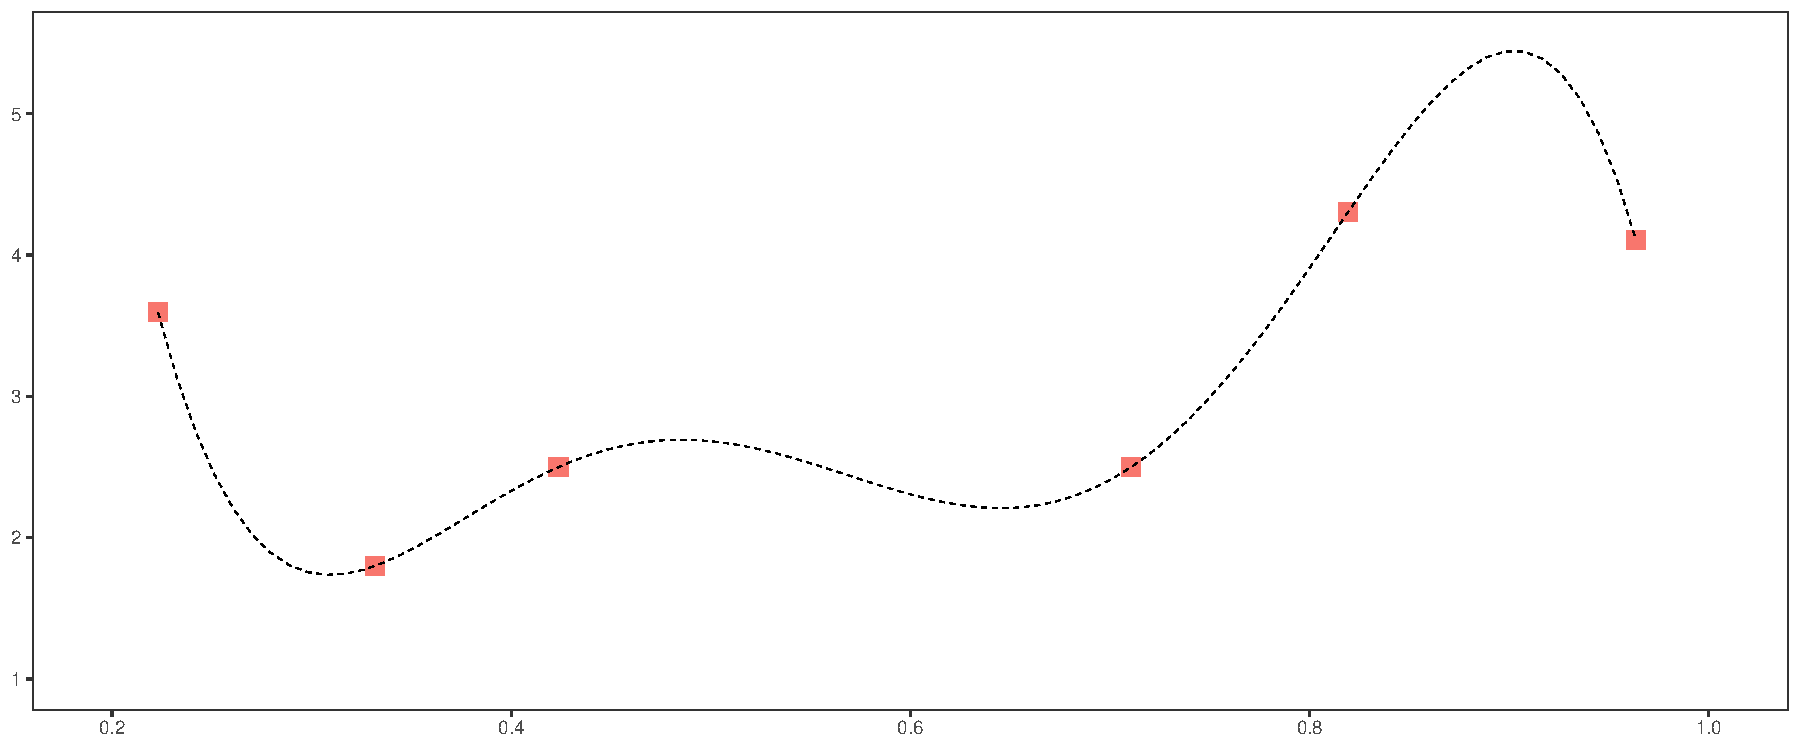
\includegraphics[scale=0.4]{figures/fig_1f.pdf}
 \end{figure}

\end{frame}

%----------------------------------------------------------------------%
\begin{frame}[fragile]
\frametitle{Overfit}


\begin{itemize}

  \item En efecto si el modelo verdadero es $y=f(x) +u$ 
  \medskip
  \item donde $f$ es un polinomio de grado $p^*$, with $E(u)=0$ and $V(u)=\sigma^2$
  \medskip
  \item con $p^*$ finito pero desconocido
  \medskip
  \item  podemos ajustar polinomios de grados crecientes $p=1,2,....$
  
  \begin{align}
  Err (  Y )  &= MSE(\hat f) + \sigma^2  \\
                 &= Bias^2(\hat f) + V(\hat f)  + Irreducible\,Error        
  \end{align}

  
\end{itemize}

\end{frame}
%----------------------------------------------------------------------%
\begin{frame}[fragile]
\frametitle{Overfit}


\begin{itemize}

  \item Sesgado ?

\end{itemize}

  \begin{align}
  \hat f(x) = X'\hat\beta=\sum_{s=0}^p x^s\hat\beta_s = x'\hat\beta  
  \end{align}

  donde $X'=(1,x,,x^2,\dots,x^p)$



\end{frame}
%----------------------------------------------------------------------%
\begin{frame}[fragile]
\frametitle{Overfit}


\begin{itemize}

  \item Varianza:
\end{itemize}

 
  \begin{align}
  V(\hat f(x) ) = V(X'\hat\beta) = \sigma^2 \frac{p}{n}
  \end{align}

 

Después de  $p^*$ aumentar la complejidad no reduce el sesgo, pero la varianza aumenta monotónicamente para  $\sigma^2$ y $n$ dados
 
\end{frame}
%----------------------------------------------------------------------%
\subsection{Overfit y Predicción fuera de Muestra}
%----------------------------------------------------------------------%
\begin{frame}[fragile]
\frametitle{Overfit y Predicción fuera de Muestra}


\begin{itemize}
  \item ML nos interesa la predicción fuera de muestra
  \medskip
  \item Overfit: modelos complejos predicen muy bien dentro de muestra, pero tienden a hacer un trabajo fuera de muestra 
  \medskip
  \item Hay que elegir el nivel adecuado de complejidad 
  \medskip
  \item Como medimos el error de predicción fuera de muestra?
  \medskip
  \item $R^2$ no funciona: se concentra en la muestra y es no decreciente en complejidad
\end{itemize}

\end{frame}

%----------------------------------------------------------------------%
\begin{frame}[fragile, noframenumbering]
\frametitle{Overfit}


        \begin{figure}[H] \centering
            \captionsetup{justification=centering}
              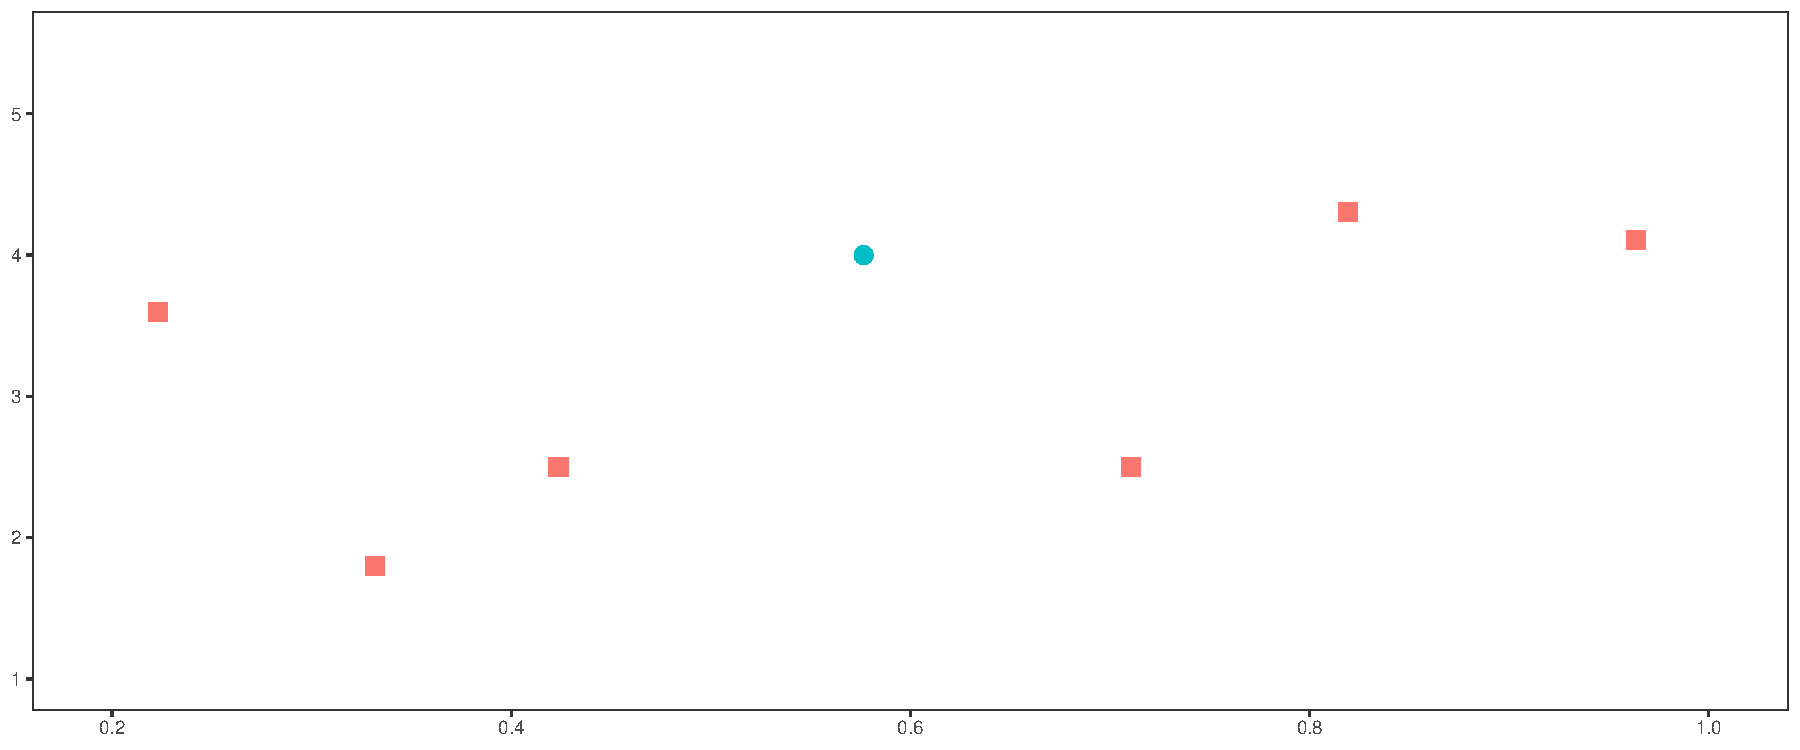
\includegraphics[scale=0.4]{figures/fig_1g.pdf}
 \end{figure}

\end{frame}


%----------------------------------------------------------------------%
\begin{frame}[fragile, noframenumbering]
\frametitle{Overfit}


        \begin{figure}[H] \centering
            \captionsetup{justification=centering}
              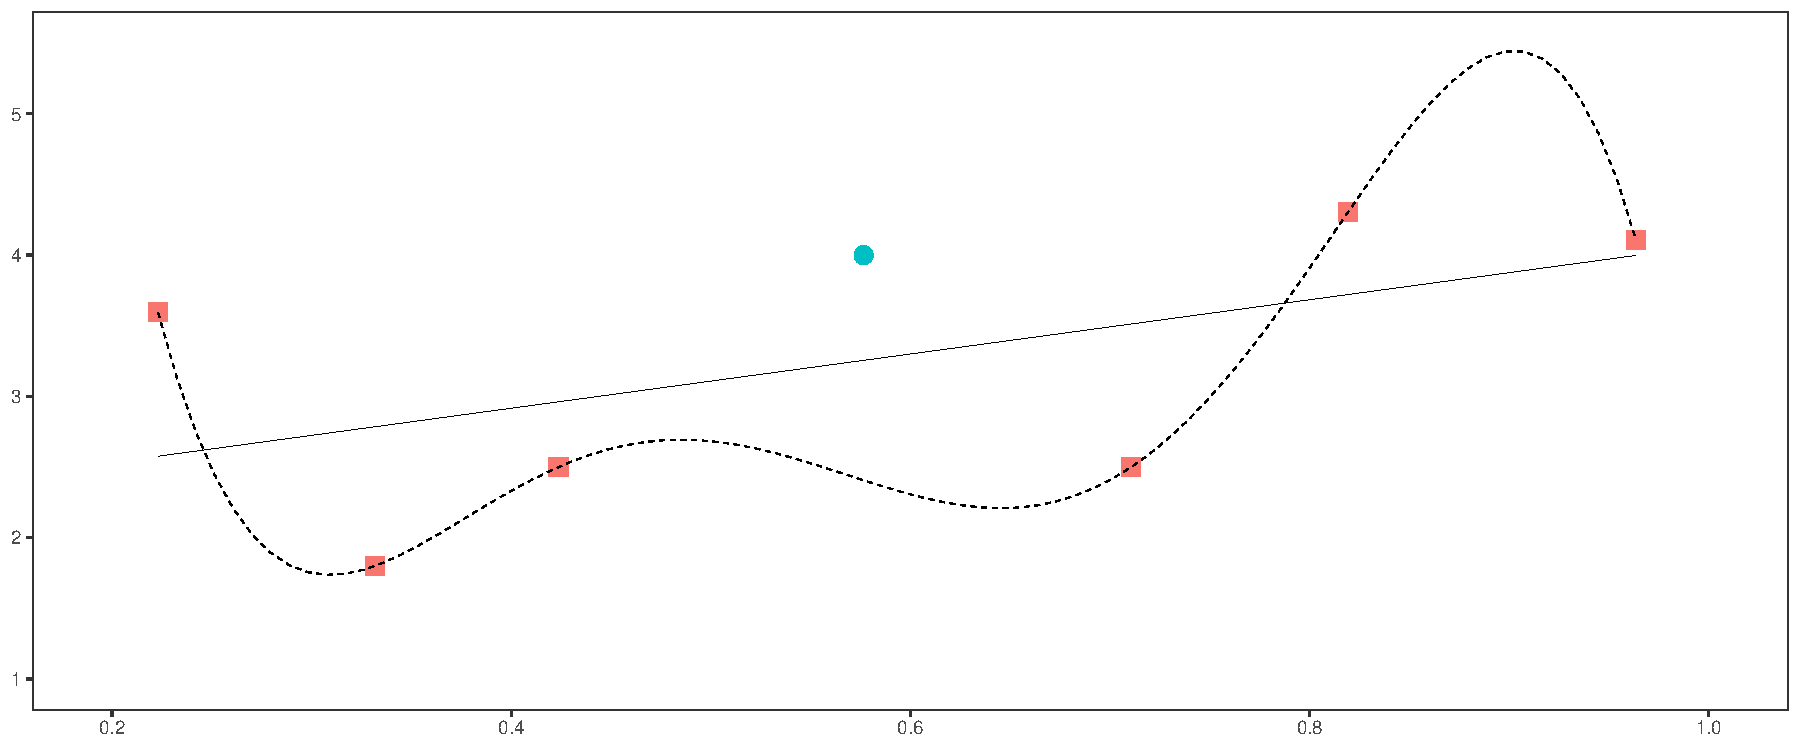
\includegraphics[scale=0.4]{figures/fig_1h.pdf}
 \end{figure}

\end{frame}
%----------------------------------------------------------------------%

%----------------------------------------------------------------------%
\subsection{AIC: Akaike Information Criterion}
%----------------------------------------------------------------------%
\begin{frame}[fragile]
\frametitle{AIC}

\begin{itemize}

\item Akaike (1969) fue el primero en ofrecer un enfoque unificado al problema de la selección de modelos.

\item Su punto de vista fue elegir un modelo del conjunto $ {f_i} $ que funcionó bien cuando se evaluó sobre la base del rendimiento de la previsión. 

\item Su criterio, que ha llegado a llamarse criterio de información de Akaike, es

\begin{align}
AIC(j) = log \left( \frac{1}{n} \sum_{i=1}^n (y_i - \hat{y} )^2\right) - p_j
\end{align}



\end{itemize}
\end{frame}

%----------------------------------------------------------------------%
\subsection{SIC/BIC: Schwarz/Bayesian Information Criterion}
%----------------------------------------------------------------------%
\begin{frame}[fragile]
\frametitle{BIC}
\begin{itemize}
\item Schwarz (1978) mostró que, si bien el enfoque $AIC$ puede ser bastante satisfactorio para seleccionar un modelo de pronóstico
\item Sin embargo, tiene la desafortunada propiedad de que es inconsistente, (cuando $n \rightarrow \infty$, tiende a elegir un modelo demasiado grande con probabilidad positiva)

\item Schwarz (1978) formalizó el problema de selección de modelos desde un punto de vista bayesiano:
\begin{align}
SIC(j) = log \left( \frac{1}{n} \sum_{i=1}^n (y_i - \hat{y} )^2\right) -\frac{1}{2} p_j log(n)
\end{align}


\end{itemize}
\end{frame}
%----------------------------------------------------------------------%
\begin{frame}[fragile]
\frametitle{AIC vs BIC}

\begin{align}
AIC(j) = log \left( \frac{1}{n} \sum_{i=1}^n (y_i - \hat{y} )^2\right)- p_j
\end{align}


\begin{align}
SIC(j) = log \left( \frac{1}{n} \sum_{i=1}^n (y_i - \hat{y} )^2\right) -  p_j \frac{1}{2} log(n)
\end{align}

\begin{itemize}
\item Note que  

\begin{align}
\frac{1}{2} log(n) > 1 \,\,\, for \,\,\, n > 8
\end{align}

 \item La penalidad de SIC es mayor que la penalidad de AIC, 
 \item SIC tiende a elegir modelos más pequeños. 
 \item En efecto, al dejar que la penalización tienda al infinito lentamente con $n$, eliminamos la tendencia de AIC a elegir un modelo demasiado grande.

\end{itemize}
\end{frame}

%----------------------------------------------------------------------%
\begin{frame}[fragile]
\frametitle{Métodos de resampleo}

\begin{itemize}
  \item Los métodos de resampleo son una herramienta indispensable de la estadística moderna.
  \medskip
  \item Estos envuelven sacar muestras aleatorias de nuestra muestra y reajustar el modelo de interés en cada muestra para obtener información adicional del modelo.
  \medskip
  \item Quizás el método más conocido por ustedes es el de bootstrap.
  \medskip
  \item Nosotros vamos a discutir la validación cruzada (cross-validation)
\end{itemize}

\end{frame}
%----------------------------------------------------------------------%
\begin{frame}[fragile]
\frametitle{Error de Prueba y de Entrenamiento}


\begin{itemize}

\item Dos conceptos importantes
\medskip
\begin{itemize}
  \item {\it Test Error}: es el error de predicción en la muestra de prueba (test)
  \medskip
  \begin{align}
    Err_{\mathcal{T}est} =MSE[(y,\hat y)|\mathcal{T}est]
  \end{align}
  \medskip
  \item {\it Training error}:es el error de predicción en la muestra de entrenamiento (training)
  \medskip
  \begin{align}
    Err_{\mathcal{T}rain} = MSE[(y,\hat y)|\mathcal{T}rain]
  \end{align}
    \end{itemize}
    \medskip
  \item Cómo elegimos $\mathcal{T}est$?
  
\end{itemize}



\end{frame}
%----------------------------------------------------------------------%
\section{ Métodos de Remuestreo}
%----------------------------------------------------------------------%
\begin{frame}[fragile]
\frametitle{Qué son los Métodos de Remuestreo?}

\begin{itemize}



\item Herramientas que implican extraer repetidamente muestras de un conjunto de entrenamiento y reajustar el modelo de interés en cada muestra para obtener más información sobre el modelo.
\medskip
\item Evaluación del modelo: estimar el error de predicción en la muestra de prueba
\medskip
\item Selección de modelo: seleccione el nivel apropiado de flexibilidad del modelo
\medskip
\item ¡Son computacionalmente costosos! Pero en estos días tenemos computadoras poderosas

\end{itemize}




\end{frame}
%----------------------------------------------------------------------%
\subsection{Enfoque de conjunto de validación}
%----------------------------------------------------------------------%
\begin{frame}[fragile]
\frametitle{Enfoque de conjunto de validación}

\begin{itemize}
\item Suponga que nos gustaría encontrar un conjunto de variables que den el menor  error de predicción en la muestra de prueba (no de entrenamiento) 
\item Si tenemos muchos datos, podemos lograr este objetivo dividiendo aleatoriamente los datos en partes de entrenamiento y validación (prueba)
\item Luego usaríamos la parte de entrenamiento para construir cada modelo posible (es decir, las diferentes combinaciones de variables) y elegimos el modelo que dio lel menor  error de predicción en la muestra de prueba
\end{itemize}

       \begin{figure}[H] \centering
            \captionsetup{justification=centering}
              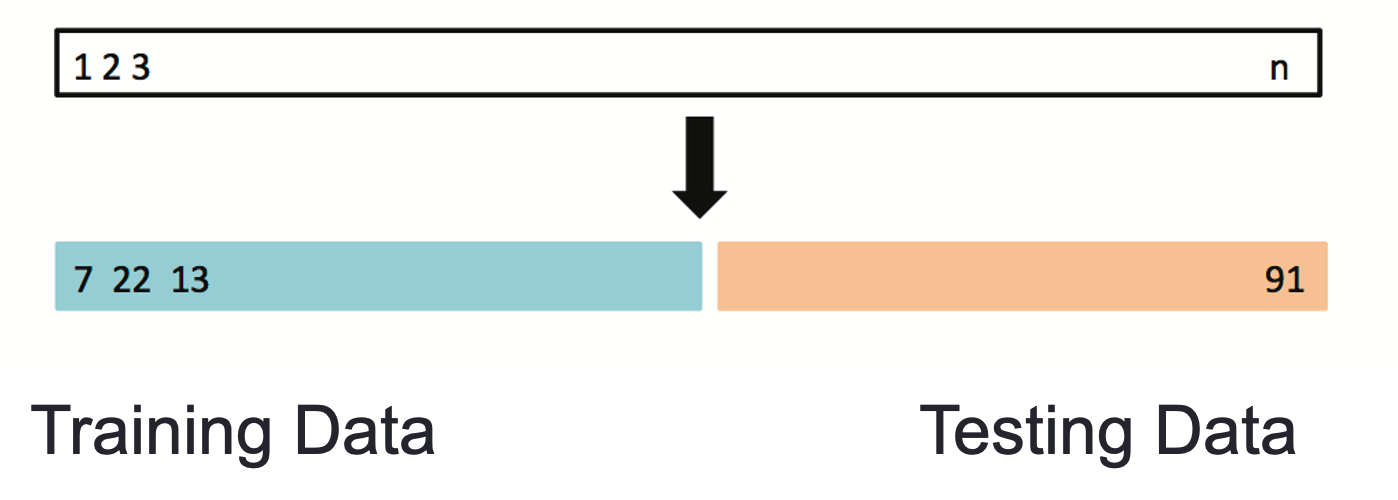
\includegraphics[scale=0.4]{figures/fig51.png}
       \end{figure}

\end{frame}

%----------------------------------------------------------------------%
\begin{frame}[fragile]
\frametitle{Enfoque de conjunto de validación}
\begin{itemize}
\item Modelo $y=f(x) +u$ donde $f$ es un polinomio de grado $p^*$. 
\scriptsize
\item Izquierda: error de predicción en la muestra de prueba para una sola partición
\item Derecha: error de predicción en la muestra de prueba para varias particiones
\item  Hay un montón de variabilidad. (Necesitamos algo mas estable)
\end{itemize}


 \begin{figure}[H] \centering
            \captionsetup{justification=centering}
              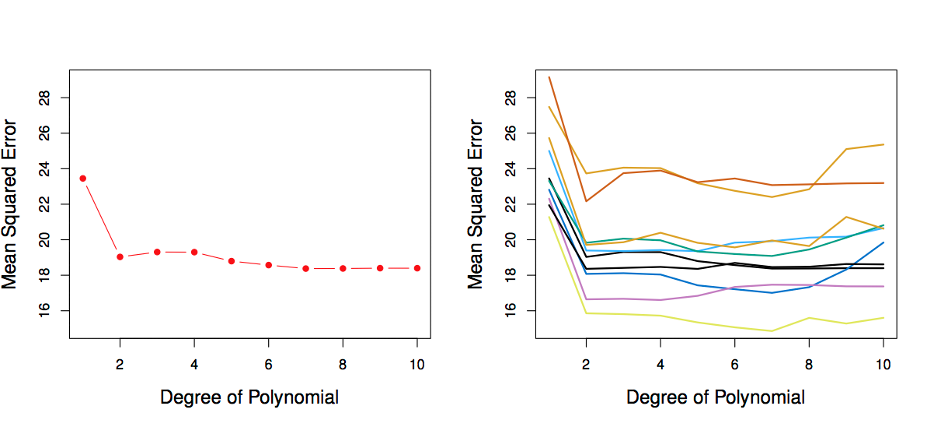
\includegraphics[scale=0.7]{figures/fig52.png}
       \end{figure}
\end{frame}
%----------------------------------------------------------------------%
\begin{frame}[fragile]
\frametitle{Enfoque de conjunto de validación}

\begin{itemize}
  \item Ventajas:
  \medskip
    \begin{itemize}
      \item Simple
      \medskip
      \item Fácil de implementar
      \medskip
    \end{itemize}
  \item Desventajas:
  \medskip
    \begin{itemize}
      \item El MSE de validación (prueba) puede ser altamente variable
      \medskip
      \item  Solo se utiliza un subconjunto de observaciones para ajustar el modelo (datos de entrenamiento). Los métodos estadísticos tienden a funcionar peor cuando se entrenan con pocas observaciones
\end{itemize}
\end{itemize}

\end{frame}
%----------------------------------------------------------------------%
\subsection{LOOCV}
%----------------------------------------------------------------------%
\begin{frame}[fragile]
\frametitle{Leave-One-Out Cross Validation (LOOCV)}

\begin{itemize}
\item Este método es similar al enfoque de validación, pero trata de abordar las desventajas de este último. 
\end{itemize}

 \begin{figure}[H] \centering
            \captionsetup{justification=centering}
              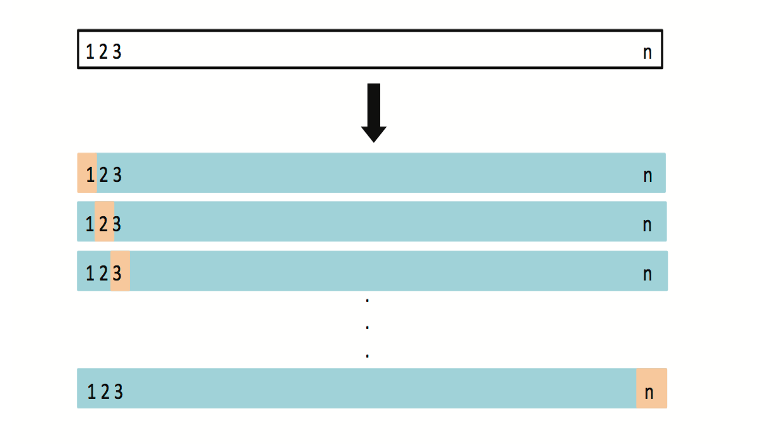
\includegraphics[scale=0.7]{figures/fig53.png}
       \end{figure}


\end{frame}
%----------------------------------------------------------------------%
\subsection{Validación cruzada en K-partes}
%----------------------------------------------------------------------%
\begin{frame}[fragile]
\frametitle{Validación cruzada en K-partes}
\begin{itemize}
\item LOOCV es computacionalmente intensivo, por lo que podemos ejecutar k-fold Cross Validation 
\end{itemize}


 \begin{figure}[H] \centering
            \captionsetup{justification=centering}
              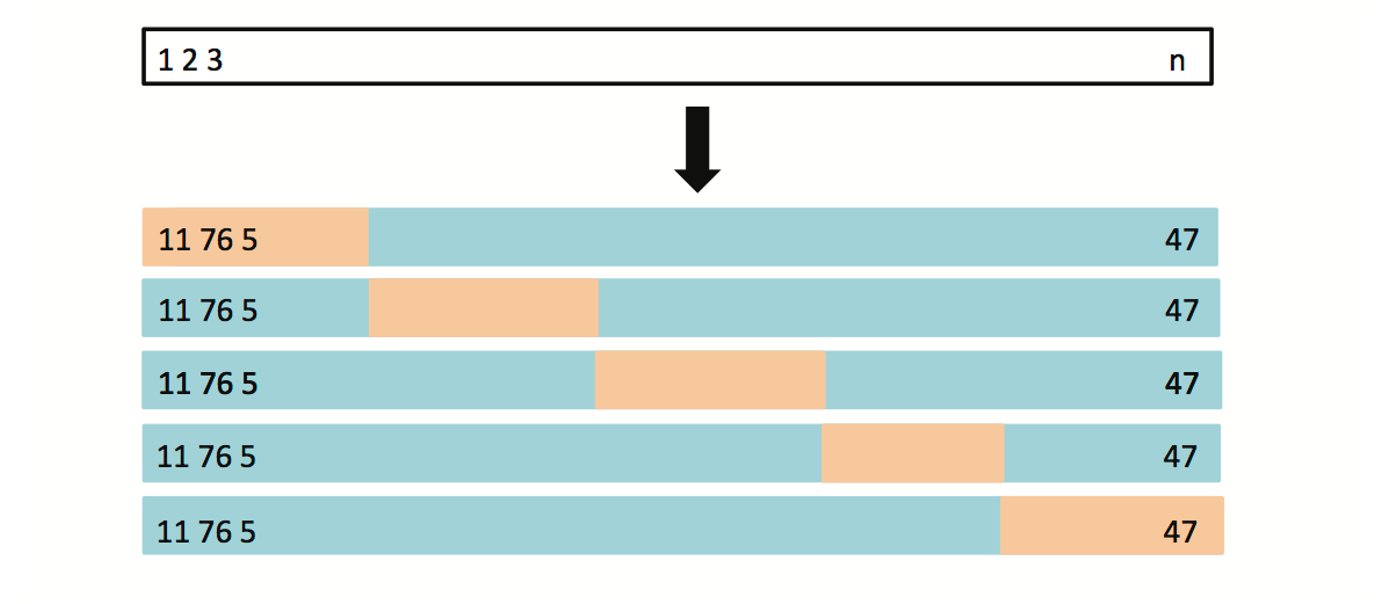
\includegraphics[scale=0.5]{figures/fig55.png}
       \end{figure}



\end{frame}
%----------------------------------------------------------------------%
\begin{frame}[fragile]
\frametitle{Validación cruzada en K-partes}

\begin{itemize}
  \item Dividir los datos en K partes $(N=\sum_{j=1}^K n_j)$
  \medskip
  \item Ajustar el modelo dejando afuera una de las partes (folds)  $\rightarrow$ $f_{-k}(x)$
  \medskip
  \item Calcular el error de predicción en la parte (fold) que dejamos afuera 
  \begin{align}
  MSE_j=\frac{1}{n_j}\sum (y_j^k-\hat y_{-j})^2
  \end{align}
  \medskip
\item Promediar

\begin{align}
CV_{(k)}= \frac{1}{k}\sum_{j=1}^k MSE_j
\end{align}
\end{itemize}

\end{frame}
%----------------------------------------------------------------------%
\begin{frame}[fragile]
\frametitle{Validación cruzada en K-partes}
\begin{itemize}
  \scriptsize
\item Izquierda: LOOCV  error 
\item Derecha: 10-fold CV 
\item LOOCV es caso especial de k-fold, donde k = n
\item Ambos son estables, pero LOOCV (generalmente) es mas intensivo computacionalmente! 
\end{itemize}

        \begin{figure}[H] \centering
            \captionsetup{justification=centering}
              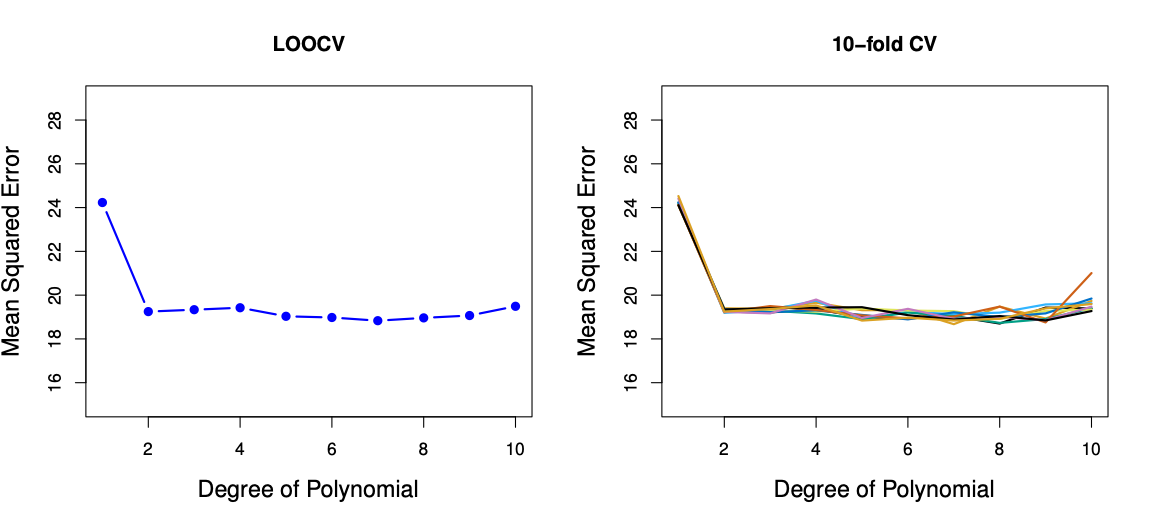
\includegraphics[scale=0.5]{figures/fig54.png}
       \end{figure}
\end{frame}


%----------------------------------------------------------------------%
\begin{frame}[fragile]
\frametitle{Validación cruzada en K-partes para selección de modelos}

\begin{itemize}
  \item Supongamos que $\alpha$ parametriza la complejidad del modelo (en nuestro ejemplo el grado del polinomio)
  \medskip
  \item Primero calculamos el CV error para un grupo de modelos ($\alpha$), y elegimos el mínimo

\end{itemize}
\begin{align}
\underset{\alpha}{min} \, CV_{(k)}(\alpha)
\end{align}

        \begin{figure}[H] \centering
            \captionsetup{justification=centering}
              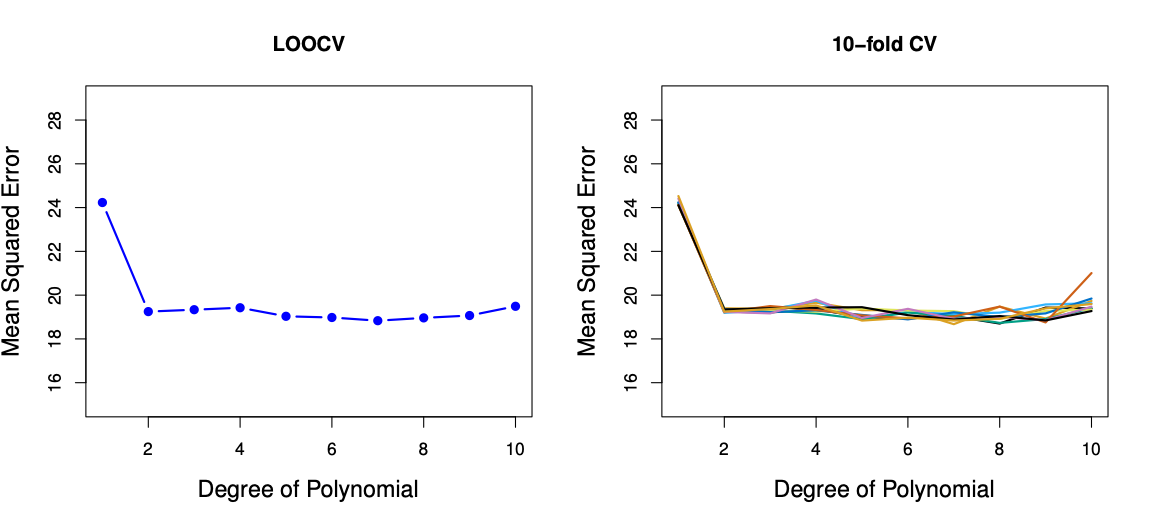
\includegraphics[scale=0.5]{figures/fig54.png}
       \end{figure}

\end{frame}

%----------------------------------------------------------------------%
\begin{frame}[fragile]
\frametitle{Trade-off Sesgo-Varianza para validación cruzada en K-partes}



\begin{itemize}
  \item Sesgo:
  \medskip
    \begin{itemize}
      \item El enfoque del conjunto de validación tiende a sobreestimar el error de predicción en la muestra de prueba (menos datos, peor ajuste)
      \item LOOCV, agrega más datos $ \rightarrow $ menos sesgo 
      \item K-fold un estado intermedio
    \end{itemize}
    \item Varianza:
    \begin{itemize}
      \item LOOCV promediamos los resultados de n modelos ajustados, cada uno está entrenado en un conjunto casi idéntico de observaciones $ \rightarrow $ altamente correlacionado
      \item K partes esta correlación es menor, estamos promediando la salida de k modelo ajustado que están algo menos correlacionados
    \end{itemize}
    \medskip
  \item Por lo tanto, existe un trade-off
  \medskip
    \begin{itemize}
      \item Tendemos a usar k-fold CV con (K = 5 y K = 10)
      \item Se ha demostrado empíricamente que producen estimaciones del error de prediccion que no sufren ni de un sesgo excesivamente alto ni de una varianza muy alta Kohavi (1995)
    \end{itemize}
\end{itemize}

\end{frame}
%----------------------------------------------------------------------%
\begin{frame}
\frametitle{Revisión \& Próximos Pasos}
  
Hoy
    \medskip
    \begin{itemize} 
        \item Dilema Sesgo/Varianza
         \medskip
         \item Sobreajuste y Selección de modelos
         \medskip
         \begin{itemize}  
         \item AIC y BIC
         \medskip
         \item Metodos de Resampleo
        \begin{itemize}  
            \item Enfoque de Validación
            \medskip
            \item LOOCV
            \medskip
            \item K-fold Cross-Validation (Validación Cruzada)
      \end{itemize}
      \end{itemize}
    




\end{itemize}



\end{frame}
%----------------------------------------------------------------------%
\section{Break}
\begin{frame}
\frametitle{}

\begin{centering}
\huge
\textcolor{andesred}{Volvemos en 15 mins con \texttt{R} }

\end{centering}

\end{frame}
%----------------------------------------------------------------------%
\section{\texttt{R para ML}}
%----------------------------------------------------------------------%
\begin{frame}
\frametitle{R para ML}

\begin{figure}[H] \centering
  \centering
  
\includegraphics[scale=0.35]{figures/baticomputer_meme.jpg}
  \\
  \tiny photo from \url{https://www.dailydot.com/parsec/batman-1966-labels-tumblr-twitter-vine/}
\end{figure}

\end{frame}
%----------------------------------------------------------------------%
%----------------------------------------------------------------------%
\end{document}
